\documentclass[]{article}

% Imported Packages
%------------------------------------------------------------------------------
\usepackage{amssymb}
\usepackage{amstext}
\usepackage{amsthm}
\usepackage{amsmath}
\usepackage{enumerate}
\usepackage{fancyhdr}
\usepackage{fullpage}
\usepackage[margin=1in]{geometry}
\usepackage{graphicx}
\usepackage{extarrows}
\usepackage{setspace}
\usepackage{caption}
\usepackage{tabularx}
\usepackage{hyperref}
\usepackage[color]{changebar}
\usepackage{placeins}
\usepackage{ulem}
%------------------------------------------------------------------------------

% Header and Footer
%------------------------------------------------------------------------------
\pagestyle{plain}  
\renewcommand\headrulewidth{0.4pt}                                      
\renewcommand\footrulewidth{0.4pt}                                    
%------------------------------------------------------------------------------

% Custom Commands
%-------------------------------------------------------------------------
\newcommand{\merlin}{\textit{Merlin }}
\newcommand{\merlins}{\textit{Merlin}'s }

\setlength\changebarsep{10pt}

\newcounter{saveenum}
\newcommand{\pauseEnum}{\setcounter{saveenum}{\value{enumi}}}
\newcommand{\resumeEnum}{\setcounter{enumi}{\value{saveenum}}}

\newcommand{\NA}{\indent\indent\emph{N/A}}
%-------------------------------------------------------------------------
% Document
%------------------------------------------------------------------------------
\begin{document}

\begin{titlepage}
\title{Deliverable \#1 - Software Requirement Specification}
\author{
	SE 3A04: Software Design II -- T2 Group 10\\
  	Jemar Jones, Rendavid Dimen, Samraj Nalwa, \\
  	Samuel Scargall, Spencer Park, Stephan Arulthasan
}
\date{February 7th, 2016}
\maketitle
\end{titlepage}

\newpage

\tableofcontents
\listoftables
\listoffigures

\section{Introduction}
\label{sec:introduction}
% Begin Section

\subsection{Purpose}
\label{sub:purpose}
% Begin SubSection
	This app is for searching and discovering songs. It gives the user a chance to find a song based on very minimal and natural inputs (e.g. beat of the song). This app is designed for the majority of music listeners with an interest in identifying tunes.
% End SubSection

\subsection{Scope}
\label{sub:scope}
% Begin SubSection
\cbstart
The app is called \merlin and will identify songs based on artist, lyric and beat. It will use these 3 criteria to try to identify the potential song using a pre-existing database. It also will utilize Google Maps to identify and display the artist’s home town. It will not give the user a song file or a link to a song file. The app interface will accept finger tapping for the beat, voice for lyrics and as well as keyboard input for the artist name. These 3 inputs will be used to identify a single song to the user. The user will not see the individual searches of the inputs only the final guess of the \merlin system.

The wide range of inputs of the \merlin system allows users to approximate their songs in a quick and easy manner without even having to know the language. The main goals of the application include having a robust voice recognition system and a very low latency tap analyser in order to provide the best possible service. If the user knows atleast one of the inputs as certain, it is very likely that the list returned to that user will include the desired song. 
\cbend
% End SubSection

\subsection{Definitions, Acronyms, and Abbreviations}
\label{sub:definitions_acronyms_and_abbreviations}
% Begin SubSection
\cbstart
\begin{table}[!ht]
\begin{tabularx}{\linewidth}{l|X}
\textbf{Term} & \textbf{Definition} \\
\hline
BPM & Beats per Minute. A measure of tempo.\\\\

speech-to-text & an in-app functionality translating sound to the text represented by the words spoken in the sound.\\\\

friend & another user of the application with whom one user of the application can share information with.\\\\

social media & the use of dedicated websites and applications to interact with other users, or to find people with similar interests to oneself.\\\\

database & a collection of information that is organized so that it can easily be accessed, managed, and updated.\\\\

beat & a main accent or rhythmic unit in music or poetry.\\\\

lyrics & the words of a song.\\\\

voice recognition & the ability of a machine or program to identify words and phrases in spoken language and convert them to a machine-readable format. (In this scope, converts to text that can be parsed by the application.)\\\\

latency & the delay between the receipt of a stimulus and the response to it.\\\\

tempo & the speed at which a passage of music is played.\\\\

API & API (application program interface) is a set of routines, protocols, and tools for building software applications. The API specifies how software components should interact.\\\\

ambient noise & noise, unintentionally created, existing in a space.
\end{tabularx}
\caption{Definitions, Acronyms, and Abbreviations}
\end{table}
\cbend
\FloatBarrier
% End SubSection

\subsection{References}
\label{sub:references}
% Begin SubSection
\cbstart

[Figure 1]Musicmachinery.files.wordpress.com, 2013. [Online]. Available: \url{https://musicmachinery.files.wordpress.com/2014/02/with_streaming_and_sharing__teens_find_ways_around_paying_for_music_-_emarketer-2.png?w=620}. [Accessed: 08- Feb- 2016].
\cbend
% End SubSection

\subsection{Overview}
\label{sub:overview}
% Begin SubSection
	The organization of this document follows the template for an SRS for scientific computing software outlined by a combination of the Volere Requirements Specification Template and the IEEE Software Requirements Specification Template. The presentation follows the standard pattern of presenting goals, theories, definitions, and assumptions. Section 2 of this document outlines the overall description of this application. This includes the product functions, user characteristics, constraints, and assumptions and dependancies. Section 3 and section 4 of this document outline the functional requirements and non functional requirements, respectively. 
% End SubSection

% End Section

\section{Overall Description}
\label{sec:overall_description}
% Begin Section

\subsection{Product Perspective}
\label{sub:product_perspective}
% Begin SubSection
The \merlin application is an Android application and as such is a component in the Android system. Merlin must therefore abide by all of the interfaces dictated for an Android application. \merlin must be written using a language and set of APIs that are accepted by the specification for an Android application. \merlin will also make use of both the microphone and touch screen peripherals of the device it is run on.
% End SubSection

\subsection{Product Functions}
\label{sub:product_functions}
% Begin SubSection
\begin{enumerate}
	\item The product will feature an innovative input method. \merlin shall be able to receive user input in the form of speech or text for artist names and/or song lyrics as well as tapping of the screen for the desired tempo (\textit{BPM}) of a song.
	\item \merlin shall use user input to search a database for songs relating to the information given.
	\item \merlin will display all relevant songs and artists to the user.
	\item The selected song's artist’s biography shall be displayed when one is selected. Home town information will also be included and shown via the Google Maps API.
	\item \merlin shall store songs and artists previously searched for by the user.
\end{enumerate}
% End SubSection

\subsection{User Characteristics}
\label{sub:user_characteristics}
% Begin SubSection
	The desired characteristics of a user of the \merlin application are as large as the domain in which the application resides. \merlin seeks to serve users who listen to music and actively try to expand their repertoire of musical choices. Users may be of any age, but \merlin shall primarily be designed for users from 13 to 40 years of age, as research (Figure \ref{fig:streaming_demographics}) shows that these age groups listen to the most music via modern platforms such as streaming services. The same research shows that males and females both stream a similar amount of content, so \merlin will target both genders.
\begin{figure}[!ht]
	\centering
	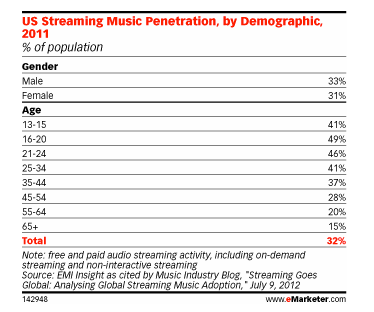
\includegraphics[scale=0.5]{StreamingByDemographic.png}
	\caption{Streaming By Demographic}
	\label{fig:streaming_demographics}
\end{figure}
% End SubSection

\subsection{Constraints}
\label{sub:constraints}
% Begin SubSection
	\merlin is subject to all constraints imposed by the Android operating system, as described in section \ref{sub:product_perspective}. The application is also subject to the physical constraints of the device it runs on, these include: device screen size, device battery life, device memory, device storage, and device processor speed. The application will also be constrained by the strength of the network connectivity used to communicate its data. Merlin will also be constrained by the environment in which the device it is run on is being used. Excessive or ambient noise near the device's microphone may impede \merlins voice recognition accuracy. Weather conditions that make it impractical for a user to use their touch screen will similarly affect the application. 
% End SubSection

\subsection{Assumptions and Dependencies}
\label{sub:assumptions_and_dependencies}
% Begin SubSection
Assumptions:
\begin{itemize}
	\item The user has a working understanding of how to use a smartphone running the Android operating system.
	\item Users of \merlin should have reasonable knowledge of the song they are searching for.
	\item When using the BPM search option, the user should have a sense of rhythm that should be similar to the beat of the song to be searched.
	\item Songs and artists being searched are relatively well known to the general populous.
\end{itemize}

\noindent Dependencies:
\begin{itemize}
	\item \merlin is run using the Android operating system. Should any changes in Android's operating system affect the application, the necessary updates to ensure the functionality of the application shall take place.
	\item The application uses the Google Maps API and should therefore be adjusted, if necessary, should any changes the the API occur
\end{itemize}
% End SubSection

\subsection{Apportioning of Requirements}
\label{sub:apportioning_of_requirements}
% Begin SubSection
The following functions may be delayed until future versions of the system:
\begin{itemize}
	\item Being able to connect with new \textit{friends}
	\item Sharing song and artist searches with your \textit{friends} on social media.
	\item Playing the song that has been searched or the most popular song of an artist tat has been searched via an external streaming service.
\end{itemize}
% End SubSection

% End Section

\section{Functional Requirements}
\label{sec:functional_requirements}
% Begin Section
\cbstart
\begin{enumerate}[{BE}1.]
	\item The user wants to find a song.
	\begin{enumerate}[{VP1}.1]
		\item Developer
			\begin{enumerate}
				\item \merlin must accept 3 search inputs: lyrics, artist and tempo.
			\end{enumerate}
		\item User
			\begin{enumerate}
				\item The user will have the option to use the app's \textit{speech-to-text} functionality to enter lyrics into the search field or type the lyrics with the devices keyboard.
				\item The user will have the option to use the app's \textit{speech-to-text} functionality to enter the artist's name into the search field or type the artist's name with the devices keyboard.
				\item The user will have the option to tap their touch screen to the beat of the song they are searching for in the tempo search field.
				\item The system must return a collection of songs and artists that \merlin finds to match the input criteria.
			\end{enumerate}
	\end{enumerate}
	\item The user wants to view their previous searches.
	\begin{enumerate}[{VP2}.1]
		\item Developer
			\begin{enumerate}
				\item \merlin must track and store all searches.
			\end{enumerate}
		\item User
			\begin{enumerate}
				\item The user must be able to view and remove searches from their saved history.
				\item The user must be able to re-execute a previous search.
			\end{enumerate}
	\end{enumerate}
	\item The user wants more information about a song result.
	\begin{enumerate}[{VP3}.1]
		\item Developer
			\begin{enumerate}
				\item \merlin must be able to retrieve and display an artist's home town on Google Maps. 
				\item \merlin must be able to retrieve and display information about the entry's artist.
				\item \merlin must be able to retrieve and display song information including title and tempo.
			\end{enumerate}
		\item User
			\begin{enumerate}
				\item Detailed information about song results can be requested by the user.
			\end{enumerate}
	\end{enumerate}
	\item The administrator wants to change the experts.
	\begin{enumerate}[{VP4}.1]
		\item Developer
			\begin{enumerate}
				\item The experts included in \merlin must be disjoint.
			\end{enumerate}
		\item Administrator
			\begin{enumerate}
				\item \merlin must support the addition or removal of an expert as requested by an administrator.
			\end{enumerate}
	\end{enumerate}
	\item An external entity wants to view a user's searches.
	\begin{enumerate}[{VP5}.1]
		\item Security
			\begin{enumerate}
				\item \merlin must encrypt all traffic being sent to an external endpoint.
			\end{enumerate}
	\end{enumerate}
\end{enumerate}
\cbend
% End Section

\section{Non-Functional Requirements}
\label{sec:non-functional_requirements}
% Begin Section
\subsection{Look and Feel Requirements}
\label{sub:look_and_feel_requirements}
% Begin SubSection

\subsubsection{Appearance Requirements}
\label{ssub:appearance_requirements}
% Begin SubSubSection
\begin{enumerate}[{LF}1. ]
	\item \sout{The product shall have a simple and easy to understand layout with 2 input methods.}
	The product shall be attractive to music listeners.
	\pauseEnum
\end{enumerate}
% End SubSubSection

\subsubsection{Style Requirements}
\label{ssub:style_requirements}
% Begin SubSubSection
\begin{enumerate}[{LF}1.]
	\resumeEnum
	\item \sout{The product shall be styled with easily readable font and no contrasting colors.}
	The product shall have the same layout as a voice recording app with a button in the middle.
\end{enumerate}
% End SubSubSection

% End SubSection

\subsection{Usability and Humanity Requirements}
\label{sub:usability_and_humanity_requirements}
% Begin SubSection

\subsubsection{Ease of Use Requirements}
\label{ssub:ease_of_use_requirements}
% Begin SubSubSection
\begin{enumerate}[{UH}1. ]
	\item The product shall be easy for a high school student to use.
	\pauseEnum
\end{enumerate}
% End SubSubSection

\subsubsection{Personalization and Internationalization Requirements}
\label{ssub:personalization_and_internationalization_requirements}
% Begin SubSubSection
\begin{enumerate}[{UH}1. ]
	\resumeEnum
	\item The product shall keep  track of the user's past searches for data analysis and improved searching.
	\pauseEnum
\end{enumerate}
% End SubSubSection

\subsubsection{Learning Requirements}
\label{ssub:learning_requirements}
% Begin SubSubSection
\begin{enumerate}[{UH}1. ]
	\resumeEnum
	\item The product shall be easy for a teenager with Android experience to learn.
	\pauseEnum
\end{enumerate}
% End SubSubSection

\subsubsection{Understandability and Politeness Requirements}
\label{ssub:understandability_and_politeness_requirements}
% Begin SubSubSection
\begin{enumerate}[{UH}1. ]
	\resumeEnum
	\item The product shall not use an offensive vocabulary or derogatory words unless contained in the proper title of the searched song.
	\item The product shall warn user of potential explicit cover arts.
	\pauseEnum
\end{enumerate}
% End SubSubSection

\subsubsection{Accessibility Requirements}
\label{ssub:accessibility_requirements}
% Begin SubSubSection
\begin{enumerate}[{UH}1. ]
	\resumeEnum
	\item The product shall be usable by anyone that has access to an android phone running an API level of 16+ (Jelly Bean).
	\item The product shall be available to download on an android phone through the developers website.
	\pauseEnum
\end{enumerate}
% End SubSubSection

% End SubSection

\subsection{Performance Requirements}
\label{sub:performance_requirements}
% Begin SubSection

\subsubsection{Speed and Latency Requirements}
\label{ssub:speed_and_latency_requirements}
% Begin SubSubSection
\begin{enumerate}[{PR}1. ]
	\item The product shall have a response time of maximum 2 seconds.
	\pauseEnum
\end{enumerate}
% End SubSubSection

\subsubsection{Safety-Critical Requirements}
\label{ssub:safety_critical_requirements}
% Begin SubSubSection
\begin{enumerate}[{PR}1. ]
	\resumeEnum
	\item The product shall not heat up the phone battery.
	\pauseEnum
\end{enumerate}
% End SubSubSection

\subsubsection{Precision or Accuracy Requirements}
\label{ssub:precision_or_accuracy_requirements}
% Begin SubSubSection
\begin{enumerate}[{PR}1. ]
	\resumeEnum
	\item The product shall have 90\% of the words of the lyric input within the song results.
	\pauseEnum
\end{enumerate}
% End SubSubSection

\subsubsection{Reliability and Availability Requirements}
\label{ssub:reliability_and_availability_requirements}
% Begin SubSubSection
\begin{enumerate}[{PR}1. ]
	\resumeEnum
	\item The product shall have the same availability as Google Maps API and database availability.
	\pauseEnum
\end{enumerate}
% End SubSubSection

\subsubsection{Robustness or Fault-Tolerance Requirements}
\label{ssub:robustness_or_fault_tolerance_requirements}
% Begin SubSubSection
\begin{enumerate}[{PR}1. ]
	\resumeEnum
	\item The product shall remain available but lacking search functionality if the database connection is lost.
	\pauseEnum
\end{enumerate}
% End SubSubSection

\subsubsection{Capacity Requirements}
\label{ssub:capacity_requirements}
% Begin SubSubSection
\begin{enumerate}[{PR}1. ]
	\resumeEnum
	\item The product must be able to cater for 1 simultaneous search.
	\item \merlin should support 100 simultaneous users searching at a given time.
	\pauseEnum
\end{enumerate}
% End SubSubSection

\subsubsection{Scalability or Extensibility Requirements}
\label{ssub:scalability_or_extensibility_requirements}
% Begin SubSubSection
	\NA
% End SubSubSection

\subsubsection{Longevity Requirements}
\label{ssub:longevity_requirements}
% Begin SubSubSection
	\begin{enumerate}[{PR}1. ]
	\resumeEnum
	\item The product must be avaiable to use until android phones stop being made.
	\pauseEnum
\end{enumerate}
% End SubSubSection

% End SubSection

\subsection{Operational and Environmental Requirements}
\label{sub:operational_and_environmental_requirements}
% Begin SubSection

\subsubsection{Expected Physical Environment}
\label{ssub:expected_physical_environment}
% Begin SubSubSection
\begin{enumerate}[{OE}1. ]
	\item The product shall be used by a person indoors under normal room temperatures and ambient noise levels.
	\pauseEnum
\end{enumerate}
% End SubSubSection

\subsubsection{Requirements for Interfacing with Adjacent Systems}
\label{ssub:requirements_for_interfacing_with_adjacent_systems}
% Begin SubSubSection
	\NA
% End SubSubSection

\subsubsection{Productization Requirements}
\label{ssub:productization_requirements}
% Begin SubSubSection
	\NA
% End SubSubSection

\subsubsection{Release Requirements}
\label{ssub:release_requirements}
% Begin SubSubSection
\begin{enumerate}[{OE}1. ]
	\resumeEnum
	\item The product shall have a new update released with every set of bug fixes. These updates will be deployed via Google Play's update service. 
	\pauseEnum
\end{enumerate}
% End SubSubSection

% End SubSection

\subsection{Maintainability and Support Requirements}
\label{sub:maintainability_and_support_requirements}
% Begin SubSection

\subsubsection{Maintenance Requirements}
\label{ssub:maintenance_requirements}
% Begin SubSubSection
\begin{enumerate}[{MS}1. ]
	\item \sout{The product shall be keeps in proper running condition at all times.}
	The product shall be updated every 3 months, or whenever an API is updated/changed.
	\pauseEnum
\end{enumerate}
% End SubSubSection

\subsubsection{Supportability Requirements}
\label{ssub:supportability_requirements}
% Begin SubSubSection
\begin{enumerate}[{MS}1. ]
	\resumeEnum
	\item The product shall have a unique email address for issues/concerns by users.
	\pauseEnum
\end{enumerate}
% End SubSubSection

\subsubsection{Adaptability Requirements}
\label{ssub:adaptability_requirements}
% Begin SubSubSection
\begin{enumerate}[{MS}1. ]
	\resumeEnum
	\item The product shall be able to adapt to the user's voice.
	\pauseEnum
\end{enumerate}
% End SubSubSection

% End SubSection

\subsection{Security Requirements}
\label{sub:security_requirements}
% Begin SubSection

\subsubsection{Access Requirements}
\label{ssub:access_requirements}
% Begin SubSubSection
\begin{enumerate}[{SR}1. ]
	\item The product shall be protected from all unauthorized attempts to read or manipulate data.
	\pauseEnum
\end{enumerate}
% End SubSubSection

\subsubsection{Integrity Requirements}
\label{ssub:integrity_requirements}
% Begin SubSubSection
\begin{enumerate}[{SR}1. ]
	\resumeEnum
	\item The product shall maintain integrity even during a data hack.
	\item The product shall not leave user data within a open directory on the phone.
	\pauseEnum
\end{enumerate}
% End SubSubSection

\subsubsection{Privacy Requirements}
\label{ssub:privacy_requirements}
% Begin SubSubSection
\begin{enumerate}[{SR}1. ]
	\resumeEnum
	\item The product shall not disclose previous user history to anyone other than the user themself.
	\pauseEnum
\end{enumerate}
% End SubSubSection

\subsubsection{Audit Requirements}
\label{ssub:audit_requirements}
% Begin SubSubSection
	\NA
% End SubSubSection

\subsubsection{Immunity Requirements}
\label{ssub:immunity_requirements}
% Begin SubSubSection
	\NA
% End SubSubSection

% End SubSection

\subsection{Cultural and Political Requirements}
\label{sub:cultural_and_political_requirements}
% Begin SubSection

\subsubsection{Cultural Requirements}
\label{ssub:cultural_requirements}
% Begin SubSubSection
\begin{enumerate}[{CP}1. ]
	\item The product shall not use any words, images or videos that will offend anyone in any part of the world excluding title's of song search responses.
	\pauseEnum
\end{enumerate}
% End SubSubSection

\subsubsection{Political Requirements}
\label{ssub:political_requirements}
% Begin SubSubSection
\begin{enumerate}[{CP}1. ]
	\resumeEnum
	\item \sout{The product shall not be linked to any political standing or party.} \NA
	\pauseEnum
\end{enumerate}
% End SubSubSection

% End SubSection

\subsection{Legal Requirements}
\label{sub:legal_requirements}
% Begin SubSection

\subsubsection{Compliance Requirements}
\label{ssub:compliance_requirements}
% Begin SubSubSection
\begin{enumerate}[{LR}1. ]
	\item The product shall obey and comply with the laws of the Data Protection Act.
	\pauseEnum
\end{enumerate}
% End SubSubSection

\subsubsection{Standards Requirements}
\label{ssub:standards_requirements}
% Begin SubSubSection
\begin{enumerate}[{LR}1. ]
	\resumeEnum
	\item The product shall comply with all data and privacy standards and specifications.
	\pauseEnum
\end{enumerate}
% End SubSubSection

% End SubSection

% End Section

\appendix

\newpage
\section{Division of Labour}
\label{sec:division_of_labour}
% Begin Section
\noindent\begin{tabular}{l l}
	\textbf{Jemar Jones} & Completion of sub sections \ref{sub:product_perspective}, \ref{sub:user_characteristics} and \ref{sub:constraints}. \\
	\textbf{Rendavid Dimen} & Completion of sub sections \ref{sub:product_functions}, \ref{sub:assumptions_and_dependencies} and \ref{sub:apportioning_of_requirements}. Supporting work on \ref{sec:functional_requirements}.\\
	\textbf{Samraj Nalwa} & Completion of section \ref{sec:non-functional_requirements}. \\
	\textbf{Samuel Scargall} & Completion of sub sections \ref{sub:purpose} and \ref{sub:scope}. \\
	\textbf{Spencer Park} & Worked on section \ref{sec:functional_requirements}, reviewed, edited and formatted the document.\\
	\textbf{Stephan Arulthasan} & Completion of sub sections \ref{sub:definitions_acronyms_and_abbreviations}, \ref{sub:references} and \ref{sub:overview}. Supporting work on \ref{sec:functional_requirements}.\\
\end{tabular}
\\

\noindent Agreement with the Division of Labour outline above:

\noindent\begin{tabularx}{\linewidth}{|l|X|}
	\hline
	\rule{0pt}{2em} \textbf{Jemar Jones} & \\
	\hline
	\rule{0pt}{2em} \textbf{Rendavid Dimen} & \\
	\hline
	\rule{0pt}{2em} \textbf{Samraj Nalwa} & \\
	\hline
	\rule{0pt}{2em} \textbf{Samuel Scargall} & \\
	\hline
	\rule{0pt}{2em} \textbf{Spencer Park} & \\
	\hline
	\rule{0pt}{2em} \textbf{Stephan Arulthasan} & \\
	\hline
\end{tabularx}
% End Section

\end{document}
%------------------------------------------------------------------------------